\clearpage
\section*{\currfilename}

\begin{figure}[H]
  \begin{center}
    \fontsize{10pt}{10pt}\selectfont
    \begin{tikzpicture}[auto, scale=1.0, every node/.style={transform shape}, node distance=1.0cm, >=latex']
      %\node[input, left of=input1, node distance=3cm] (input1) {};
      \node[squareblock, minimum height=1cm, minimum width=2cm] (block1){\shortstack[c]{Adaptive\\Controller}};
      \node[squareblock, below of=block1, node distance=1.5cm, minimum height=1cm, minimum width=2cm] (block2){\fontsize{14pt}{14pt}\selectfont$\theta(t)$};
      \node [right of=block1,draw=black, anchor=west,node distance=2.0cm, minimum width=2cm, inner sep= 0mm, label=below:{\shortstack[c]{\bf Nonlinear Equations\\ \bf of Motion}}] (block3) {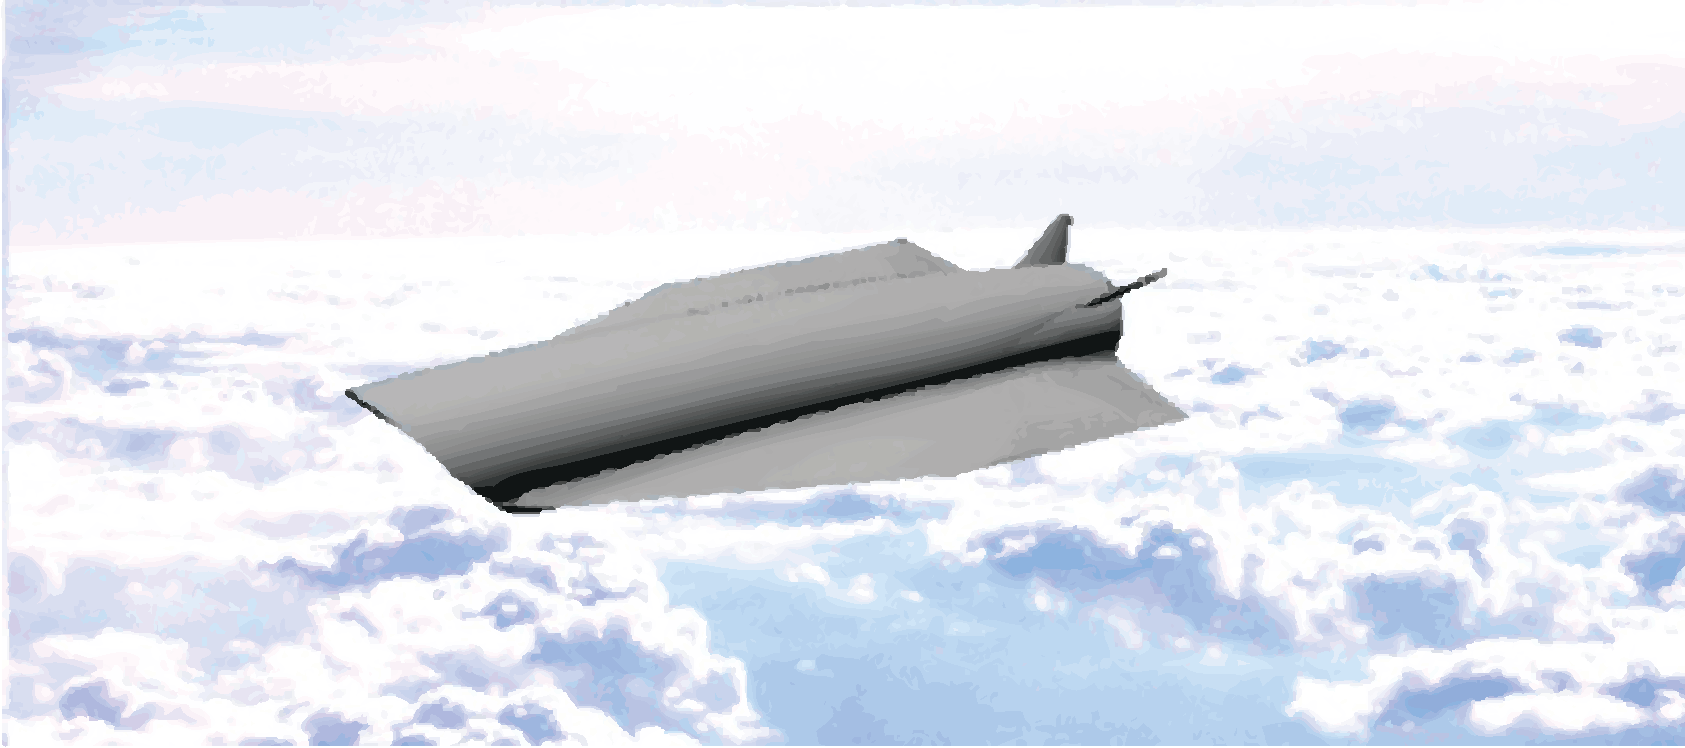
\includegraphics[width=4cm]{../fig/ghvclouds.pdf}};
      \node[squareblock, minimum height=1cm, minimum width=2cm, right of=block3, node distance=4.0cm] (block4) {\shortstack[c]{Error \\ Generator}};
      \node[output, right of=block4,node distance=2.0cm] (output1) {};
      \node[input, below of=block2, node distance=1.5cm] (input2) {};
      %\draw[->](input1) -- (block1);
      \draw[->](input2) -- node[pos=0.5]{$e$, $x$, $\Gamma$}(block2);
      \draw[->](block2) -- (block1);
      \draw[->](block1) -- (block3);
      \draw[->](block3) -- (block4);
      \draw[->](block4) --  node[pos=0.8]{$e$}(output1);
    \end{tikzpicture}
    \caption{Baseline plus adaptive control block diagram \label{fig.baseplusadaptiveblock}}
  \end{center}
\end{figure}
